\documentclass[10pt,
% a4paper,
%twocolumn,
fleqn,
%landscape, 
% papersize,
dvipdfmx,
uplatex
]{jsarticle}



\def\maru#1{\textcircled{\scriptsize#1}}%丸囲み番号

% \RequirePackage[2020/09/30]{platexrelease}

%太字設定
\usepackage[deluxe]{otf}

\usepackage{emathEy}

\usepackage[g]{esvect}

%定理環境
\usepackage{emathThm}
%\theoremstyle{boxed}
\theorembodyfont{\normalfont}
\newtheorem{Question}{問題}[subsection]
\newtheorem{Q}{}[subsection]
\newtheorem{question}[Question]{}
\newtheorem{quuestion}{}[subsection]

%セクション,大問番号のデザイン
\renewcommand{\labelenumi}{(\arabic{enumi})}
\renewcommand{\theenumii}{\alph{enumii})}
\renewcommand{\thesection}{第\arabic{section}章}

%用紙サイズの詳細設定
\usepackage{bxpapersize}
\papersizesetup{size={80mm,45mm}}
\usepackage[top=0.7zw,bottom=0truemm,left=3truemm,right=133truemm]{geometry}
\usepackage[dvipdfmx]{graphicx}

%余白など
\usepackage{setspace} % 行間
\setlength{\mathindent}{1zw}
\setlength\parindent{0pt}


%色カラーに関する設定
\usepackage{color}
\definecolor{shiro}{rgb}{0.95703125,0.87109375,0.7421875}
\definecolor{kin}{rgb}{0.95703125,0.87109375,0.7421875}
\definecolor{orange}{rgb}{1,0.7,0.2}
\definecolor{bradorange}{rgb}{1,0.5,0}
\color{kin}
% \pagecolor{hukamido}

\usepackage{at}%図の配置
% \usepackage{wallpaper}

\begin{document}




\at(0cm,0cm){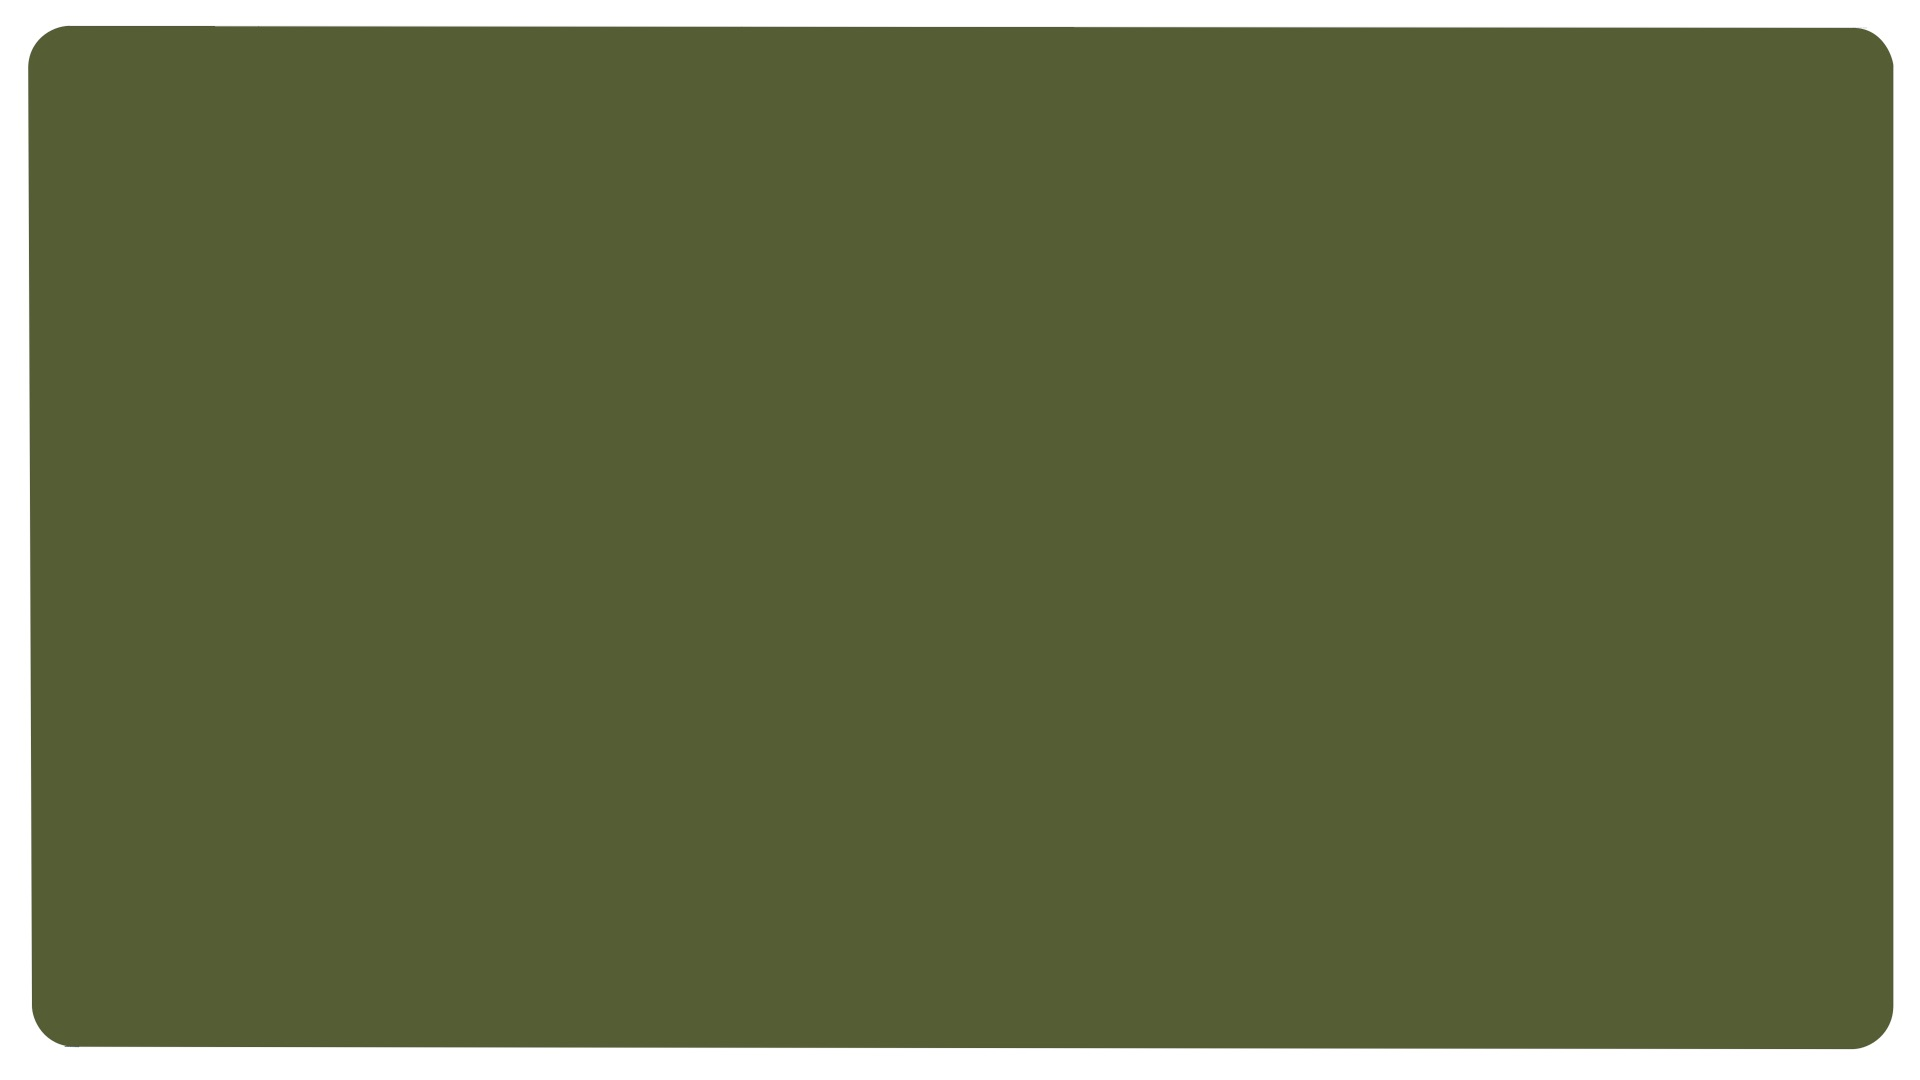
\includegraphics[width=8cm,bb=0 0 1920 1080]{./media_local/smart_background/三角比.jpeg}}
{\color{orange}\bf\boldmath\LARGE\underline{内接円と外接円の半径}}\vspace{0.3zw}

\large 
\bf\boldmath 問.$\triangle \text{ABC}$において,\\
\hfill $\text{AB}=5,\;\text{BC}=7,\;\text{AC}=8$のとき,

\huge
内接円の半径$r$と外接円の半径$R$を求めよ.
\at(7.2cm,0.2cm){\small\color{bradorange}$\overset{\text{三角比}}{\text{典型}}$}


\newpage



\at(0cm,0cm){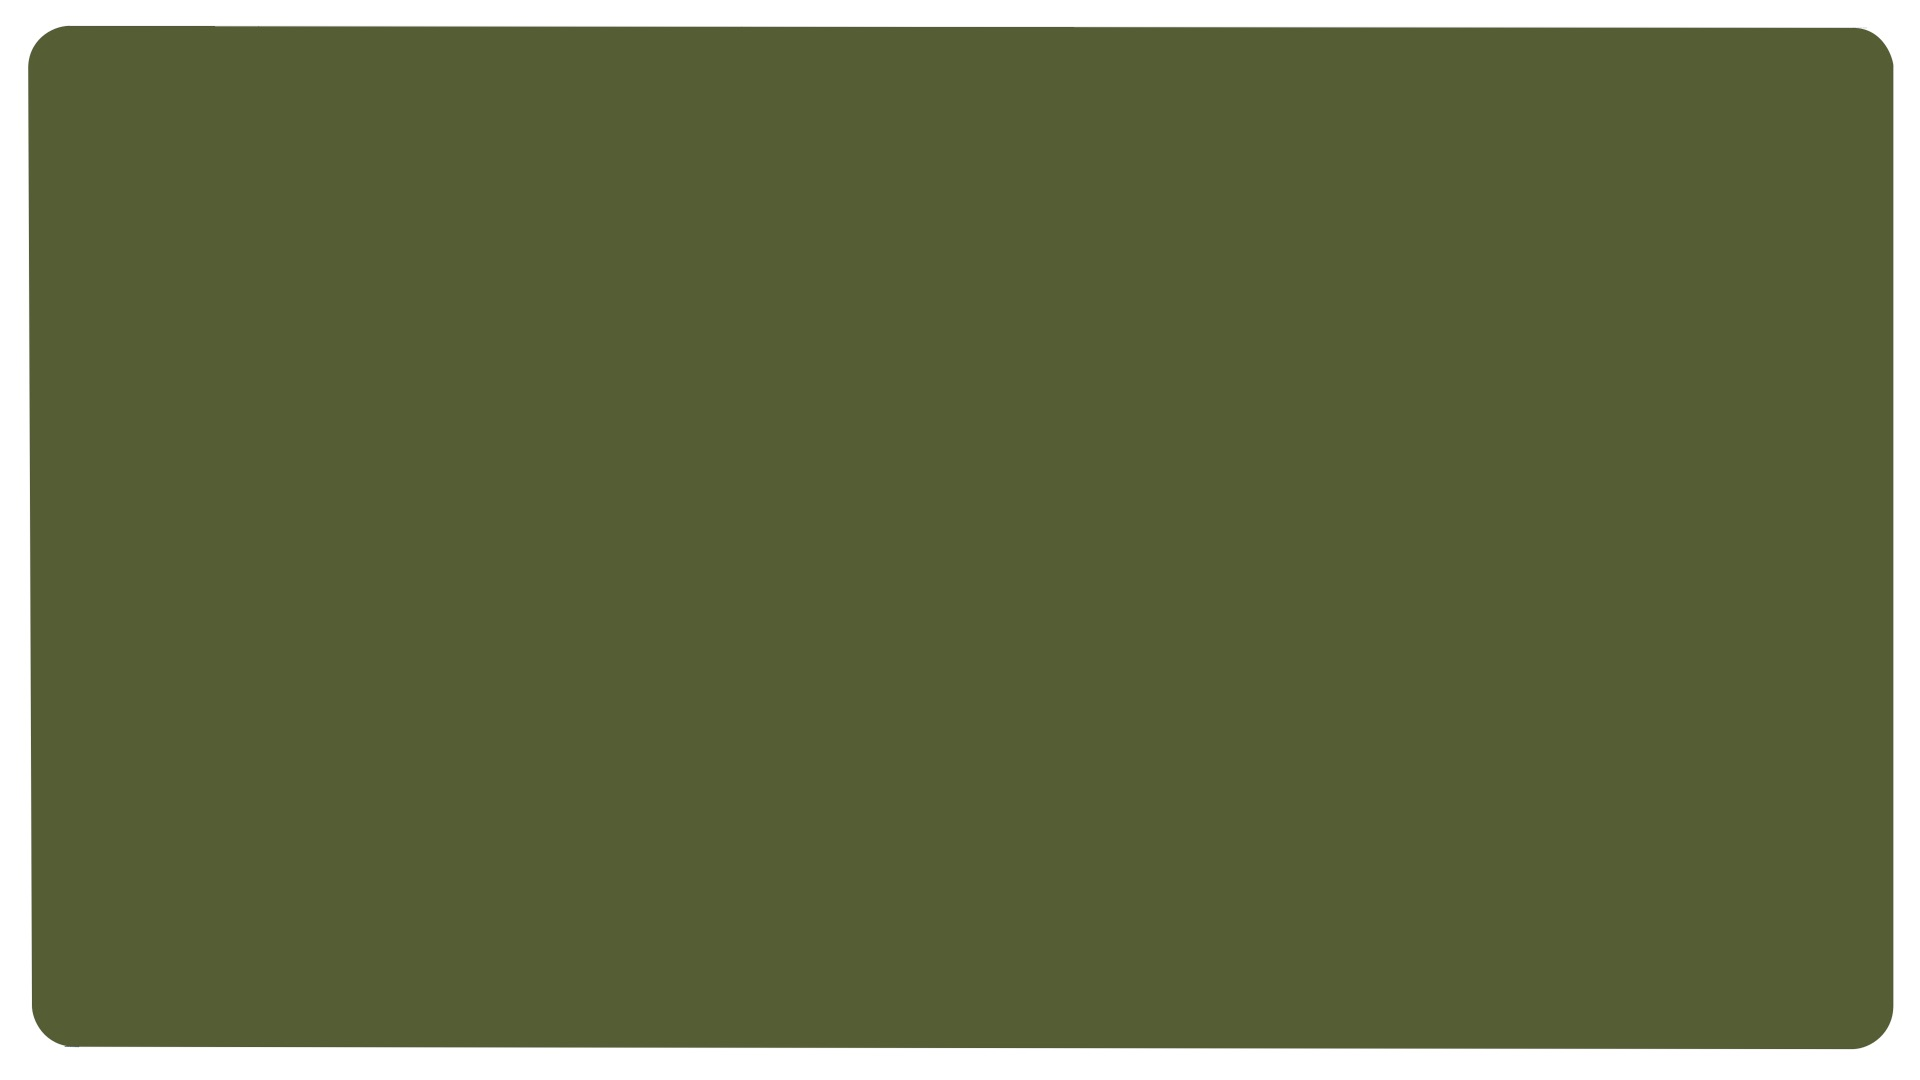
\includegraphics[width=8cm,bb=0 0 1920 1080]{./media_local/smart_background/三角比.jpeg}}
{\color{orange}\bf\boldmath\LARGE\underline{内角二等分線の長さ}}\vspace{0.3zw}

\scriptsize 
\bf\boldmath 問.$\triangle \text{ABC}$において,
\small 
$\text{AB}=5,\;\text{AC}=8,\;\angle \text{A}={60}\DEG $

\LARGE
$\angle \text{A}$の二等分線が辺$\text{BC}$と交わる点を$\text{D}$とするとき,

\Large
\hfill 線分$\text{AD}$の長さを求めよ.
\at(7.2cm,0.2cm){\small\color{bradorange}$\overset{\text{三角比}}{\text{典型}}$}


\newpage



\at(0cm,0cm){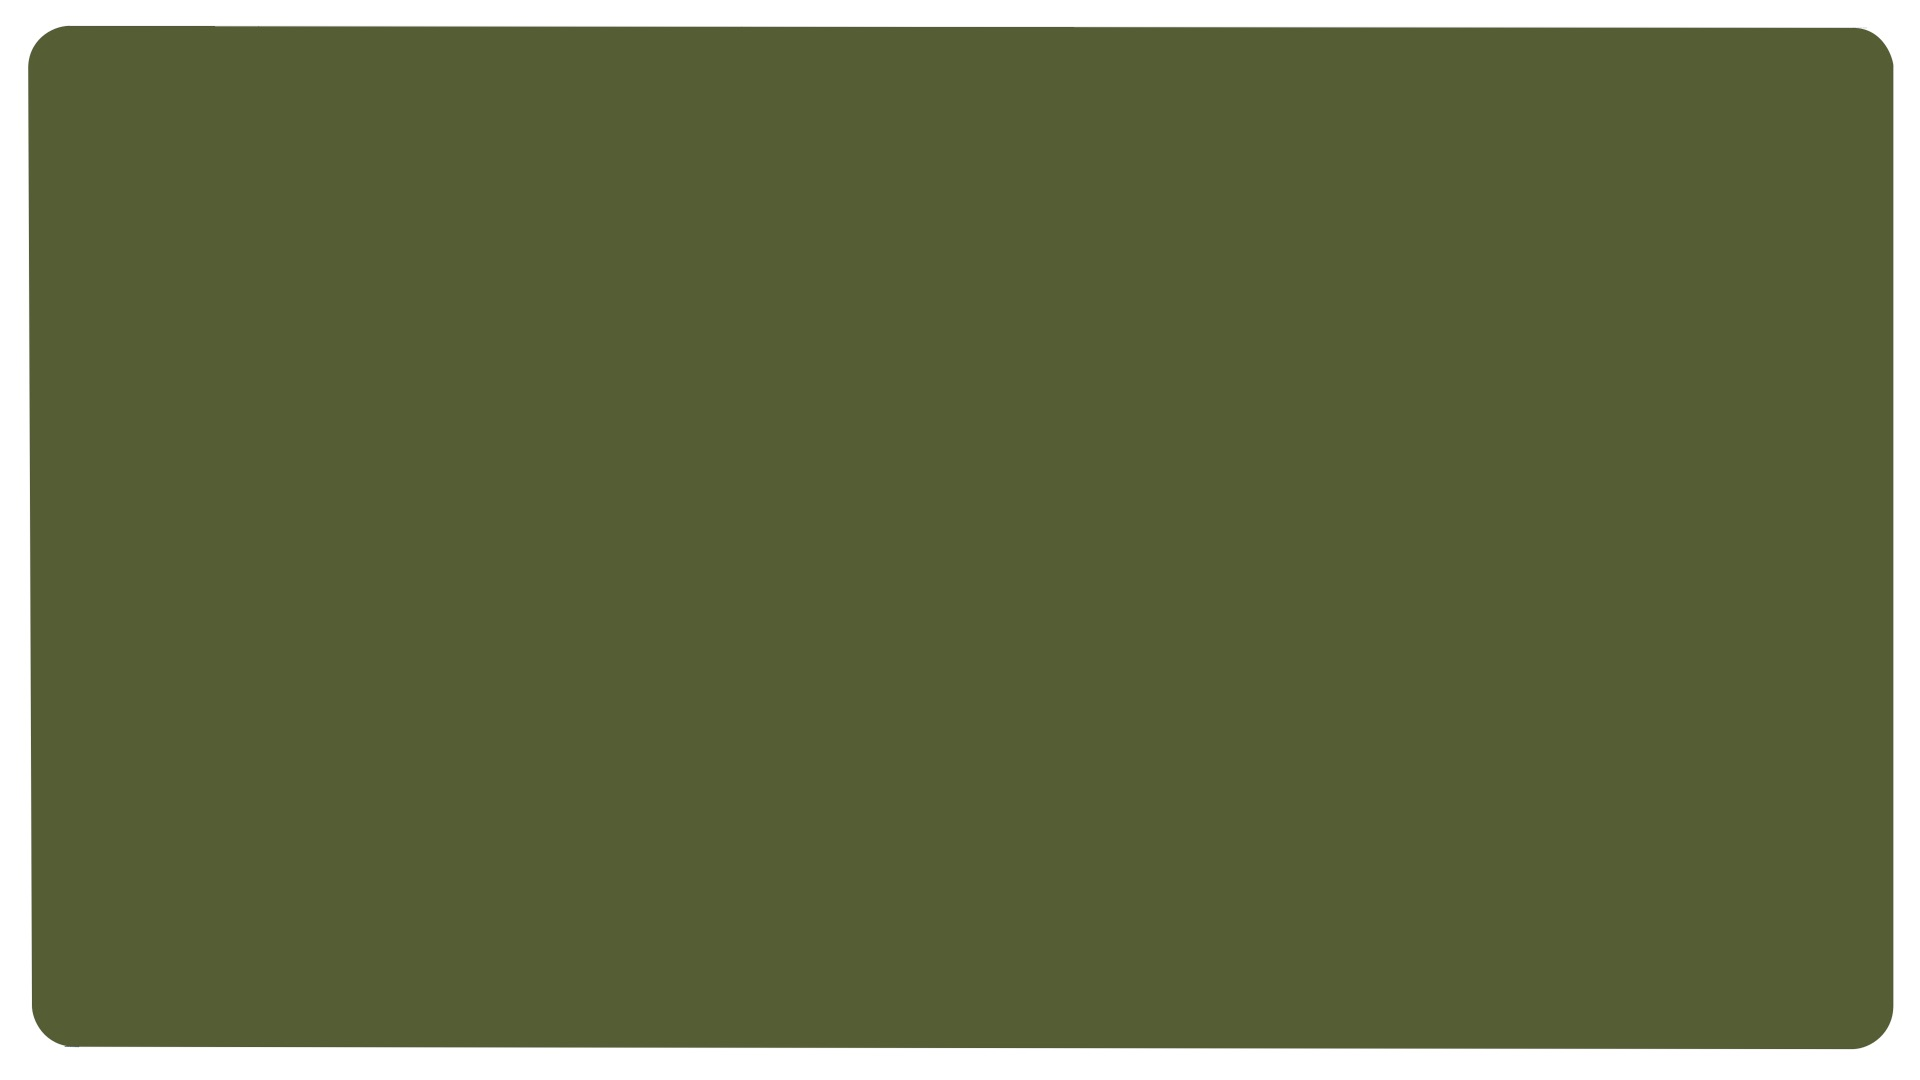
\includegraphics[width=8cm,bb=0 0 1920 1080]{./media_local/smart_background/三角比.jpeg}}
{\color{orange}\bf\boldmath\Large\underline{三角形の内角の$\sin$の比}}\vspace{0.5zw}

\LARGE 
\bf\boldmath \hspace{-0.3zw}$\bunsuu{5}{{}\sin A}=\bunsuu{7}{{}\sin B}=\bunsuu{8}{{}\sin C}\vspace{0.7zw}$

\Large
である$\triangle \text{ABC}$の最小角を$\theta$とするとき,$\cos \theta$の値を求めよ.
\at(7.2cm,0.2cm){\small\color{bradorange}$\overset{\text{三角比}}{\text{典型}}$}


\newpage



\at(0cm,0cm){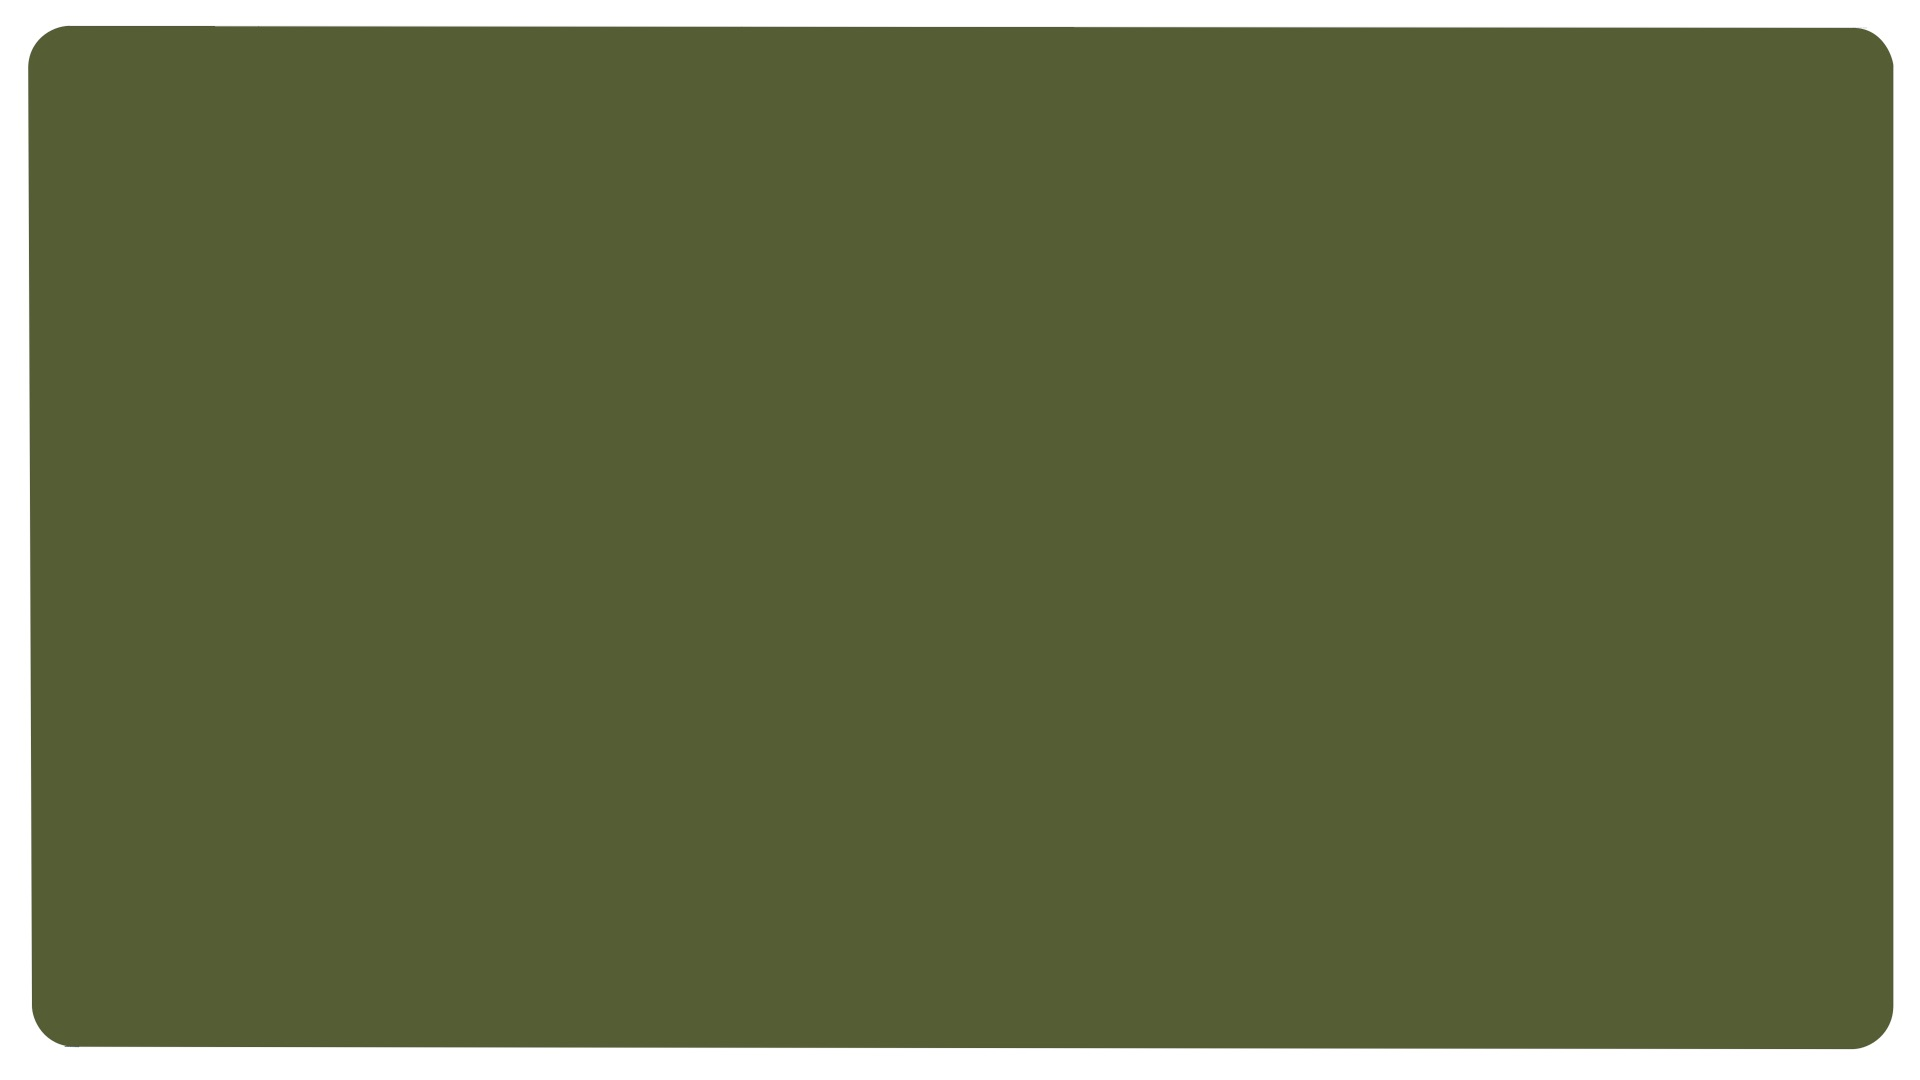
\includegraphics[width=8cm,bb=0 0 1920 1080]{./media_local/smart_background/三角比.jpeg}}
{\color{orange}\bf\boldmath\LARGE\underline{三角形の形状決定}}\vspace{0.3zw}

\LARGE 
\bf\boldmath 問.次の等式を満たす\\$\triangle \text{ABC}$はどのような形か.

\Large
\vspace{0.3zw}
\hspace{0.0zw}$a^2\cos A\sin B=b^2\cos B\sin A\vspace{0.3zw}$


\at(7.2cm,0.2cm){\small\color{bradorange}$\overset{\text{三角比}}{\text{典型}}$}


\newpage



\at(0cm,0cm){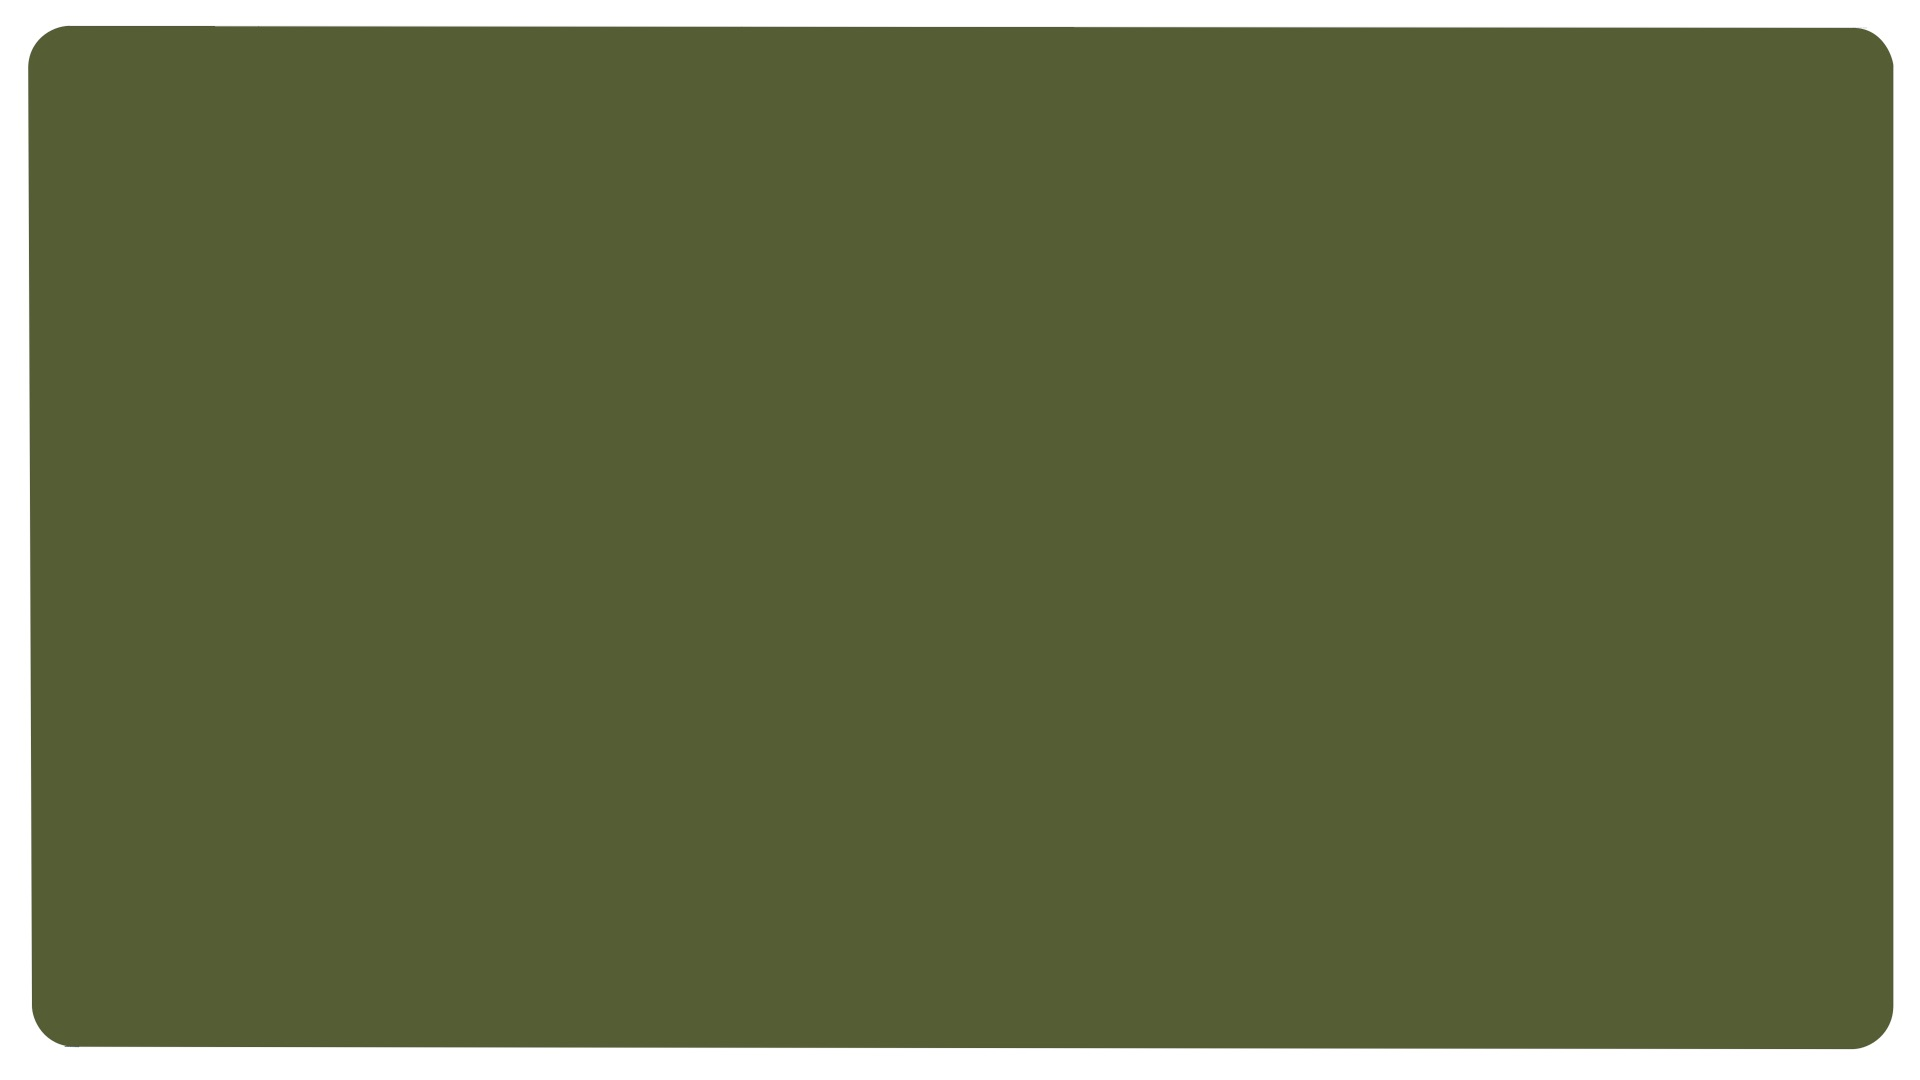
\includegraphics[width=8cm,bb=0 0 1920 1080]{./media_local/smart_background/三角比.jpeg}}
{\color{orange}\bf\boldmath\Large\underline{円に内接する四角形の面積}}\vspace{0.3zw}

\normalsize 
\bf\boldmath 問.円$O$に内接する四角形$\text{ABCD}$が\\
\hspace{0.3zw}$\text{AB}=2,\;\text{BC}=3,\;\text{CD}=1,\;\angle \text{ABC}={60}^\circ$\\
を満たしている.\\
\large
(1)  円$O$の半径$R$を求めよ.\\
(2)  四角形$\text{ABCD}$の面積$S$を求めよ.\\

\at(7.2cm,0.2cm){\small\color{bradorange}$\overset{\text{三角比}}{\text{応用}}$}


\end{document}

